\documentclass{beamer}
\usepackage{beamerthemesplit}
\usepackage{color,colortbl}
\usepackage{amsfonts}
\usepackage{marvosym} % \MVRIGHTarrow
\usepackage{multimedia}
\usepackage{animate}
\usepackage{xmpmulti}
\usepackage{wrapfig}
\usepackage{tikz}
\usepackage{graphicx}
\usepackage{multicol}


%\setlength{\textwidth}{15cm}           %Sets the width of the printable area of the page to 15cm
%\setlength{\topmargin}{0cm}            %Space from the toprule to the top of the text (first line) to 0 cm.
%\setlength{\footskip}{0cm}               %Space from the bottom of the text to the footnote (or footrule) to 0 cm.
\setlength{\marginparwidth}{0cm}   
\setlength{\columnsep}{0cm}
%\newlist{arrowlist}{itemize}{1}
%\setlist[arrowlist]{label=$\Rightarrow$
\setbeamertemplate{caption}{\insertcaption} 

\definecolor{cvggreen}{RGB}{4,71,79}
\definecolor{LRed}{rgb}{1,.8,.8}

\mode<presentation>
{
%Darmstadt
\usetheme[compress]{Amsterdam}
}

\title{\textsc{\textbf{Marchiatura digitale di sequenze video stereoscopiche a disparit\`{a} coerente }}}
\author{\textsc{Benedetta Barbetti,\\ 
		Michaela Servi}}


\institute{\begin{tabular}{l c l} 
Relatori:      & \hspace{5cm} & Correlatori: \\
Alessandro Piva  & \hspace{5cm}  & Pasquale Ferrara\\
Carlo Colombo & \hspace{5cm}  & Francesca Uccheddu \\
\end{tabular}\\
\vspace{1em}Tesi Magistrale di Ingegneria Informatica \\Universit\`{a} degli Studi di Firenze }
\date{\tiny{10 Dicembre 2015}}

\begin{document}

{\usebackgroundtemplate{\tikz\node[opacity=0.1] {
\includegraphics[width=\paperwidth]{./img/logo.png}};}
\begin{frame}
\titlepage
\end{frame}
}

\begin{section}{Introduzione}
\subsection{Video Stereoscopici}

\begin{frame}[t]{\textsc{Contesto}}
\centering
Numerose applicazioni di elaborazione di immagini e video richiedono esplicite informazioni sulla \textbf{profondit\`{a}} della scena. La \textbf{stereoscopia} permette di ottenere queste informazioni.
\setlength{\columnsep}{0cm}
\begin{columns}
\begin{column}{4cm}
\begin{center}
\setbeamertemplate{blocks}[rounded][shadow=false]
	\setbeamercolor{block body}{use=structure,fg=black,bg=lightgray} 	
\begin{block}{Campi applicativi}
		\begin{itemize}
			\item \small{Medicina} 
			\item Robotica
			\item Tracking
			\item Industria manifatturiera
			\item Cinema
		\end{itemize}	
	\end{block}
\end{center}
\end{column}
\begin{column}{6cm}
\begin{figure}
\centering
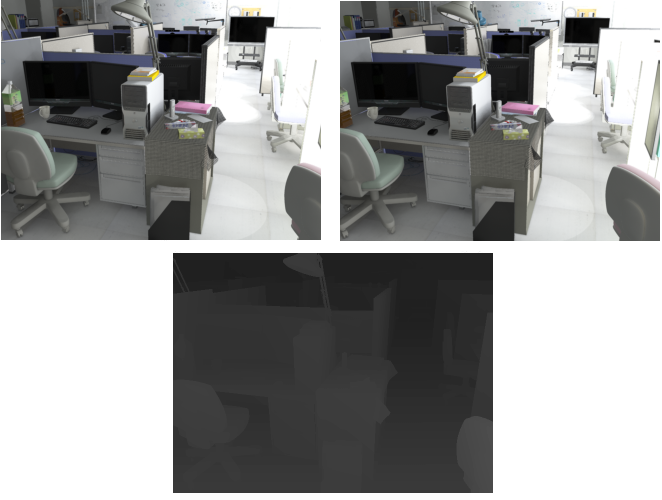
\includegraphics[width=1\linewidth]{./img/track.png}
\end{figure}
\end{column}
\end{columns}
\end{frame}

% % % % % % % % % % FRAME % % % % % % % % % % % % %

\begin{frame}[t]{\textsc{Stereoscopia}}
\vspace{-1em}
\begin{center}
	\setbeamertemplate{blocks}[rounded][shadow=false]
	\setbeamercolor{block title}{use=structure,fg=black,bg=lightgray} 
	\setbeamercolor{block body}{use=structure,fg=black,bg=lightgray} 		
\begin{block}{}
	\center Tecnica di realizzazione e visione di immagini e filmati, atta a trasmettere una illusione di \textbf{tridimensionalit\`{a}}
	\end{block}
\end{center}
\begin{center}
\vspace{-0.3em}
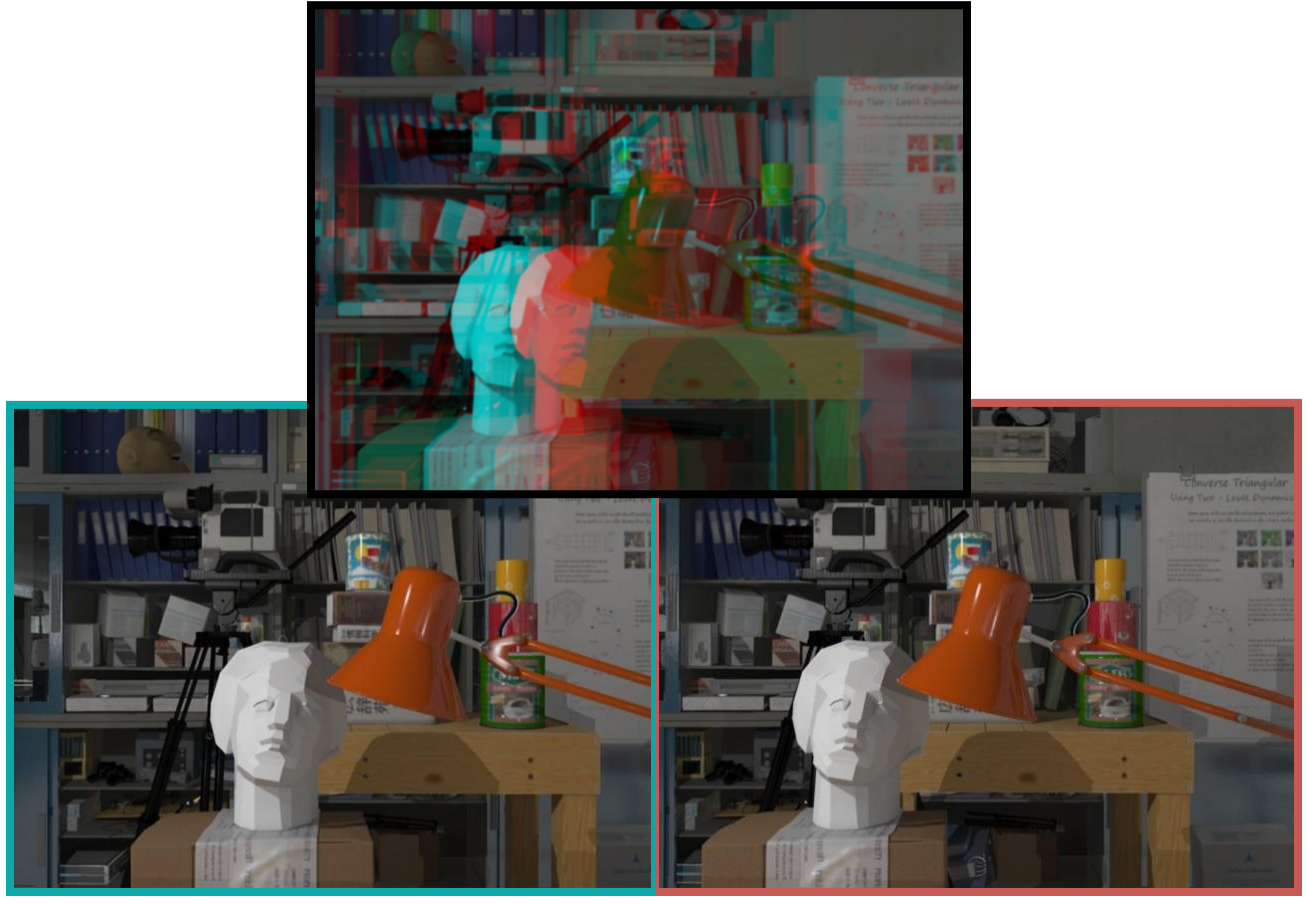
\includegraphics[width=0.7\linewidth]{./img/stereo.png}
\end{center}
\end{frame}


% % % % % % % % % % FRAME % % % % % % % % % % % % %


\begin{frame}[t]{\textsc{Video Stereoscopici}}
\setbeamertemplate{blocks}[rounded][shadow=false]
\setbeamercolor{block title}{use=structure,fg=black,bg=lightgray} 
\setbeamercolor{block body}{use=structure,fg=black,bg=lightgray} 	
	\vspace{-0.5em}
	\begin{center}
		\setbeamertemplate{blocks}[rounded][shadow=false]
		\setbeamercolor{block title}{use=structure,fg=black,bg=lightgray} 
		\setbeamercolor{block body}{use=structure,fg=black,bg=lightgray} 		
	\begin{block}{}
		\center Il \textbf{video stereoscopico} \`{e} ottenuto inquadrando la stessa scena da due \textbf{punti di vista diversi}
		\end{block}
	\end{center}
\begin{center}
\movie[width=8cm,height=5cm,autostart,loop,poster]{}{./img/alice.mp4}
\end{center}
\end{frame}

% % % % % % % % % % FRAME % % % % % % % % % % % % %

\begin{frame}[t]{\textsc{Dispositivi di ripresa e visualizzazione}}
\vspace{-0.3em}
\begin{columns}
\begin{column}{5cm}
\begin{center}
\setbeamertemplate{blocks}[rounded][shadow=false]
	\setbeamercolor{block body}{use=structure,fg=black,bg=lightgray} 
	\setbeamerfont{block body}{size=\tiny}	
\begin{block}{Sistema di ripresa stereo}
		\begin{itemize}
			\item  \small{Due telecamere sincronizzate
			\item Correttamente allineate
			\item Stessi parametri}
		\end{itemize}	
	\end{block}
\end{center}
\centering
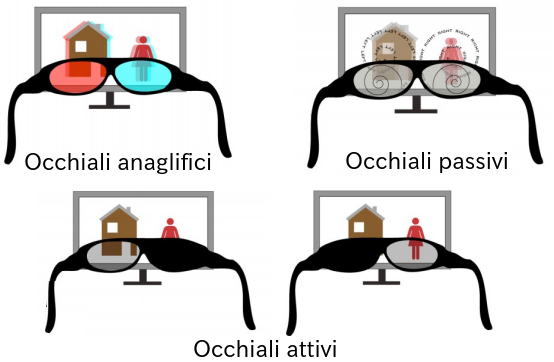
\includegraphics[width=1\linewidth]{./img/display.png}
\end{column}
\begin{column}{5cm}
\centering
\vspace{0.7em}
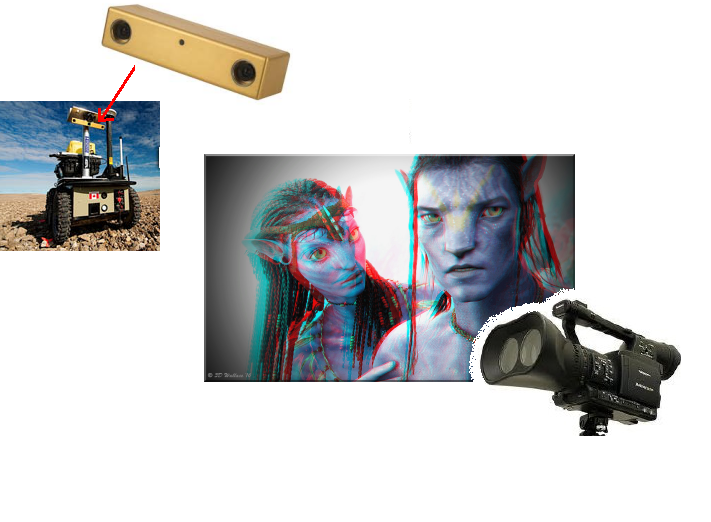
\includegraphics[width=1\linewidth]{./img/camere.png}
\vspace{-2.8em}
\begin{center}
\setbeamertemplate{blocks}[rounded][shadow=false]
	\setbeamercolor{block body}{use=structure,fg=black,bg=lightgray} 		
\begin{block}{Sistema di riproduzione}
		\begin{itemize}
			\item  \small{\textbf{Attivo}: lenti sincronizzate con il televisore
			\item \textbf{Passivo}: lenti diversamente polarizzate
			\item \textbf{Anaglifico}: lenti passive con filtri di colore diverso}
		\end{itemize}	
	\end{block}
\end{center}
\end{column}
\end{columns}
\end{frame}

% % % % % % % % % % FRAME % % % % % % % % % % % % %


\begin{frame}[t]{\textsc{Necessit\`{a} di una protezione}}
\vspace{1em}
\begin{itemize}
\item Autenticazione
\item Copyright 
\item Individuazione di falsificazioni e alterazioni

\end{itemize}
 \hspace{50 mm}$\mathbb{\Downarrow}$
\setbeamertemplate{blocks}[rounded][shadow=false]
 
\setbeamercolor{block body}{use=structure,fg=black,bg=lightgray}
\begin{block}{\centering WATERMARKING}
\center \small{\textbf{Inserimento} di \textbf{informazione} aggiuntiva in contenuti multimediali in modo \textbf{trasparente} e \textbf{robusto}\\
%\begin{itemize}
%\item Diversit\`{a} della coppia stereo 
%\item Scarsit\`{a} di soluzioni in letteratura
%\end{itemize}
}
\end{block}
 \hspace{50 mm} $\mathbb{\Downarrow}$\\
\centering nuove tecniche adatte alla diversit\`{a} della coppia stereo


\end{frame}





% % % % % % % % % % FRAME % % % % % % % % % % % % %


\begin{frame}[t]{\textsc{Obiettivo}}
\vspace{0.5em}
\begin{center}
 \setbeamertemplate{blocks}[rounded][shadow=false]
 	\setbeamercolor{block title}{use=structure,fg=black,bg=lightgray} 
 	\setbeamercolor{block body}{use=structure,fg=black,bg=lightgray}
 \begin{block}{}
 \center \large{Implementazione di un \textbf{sistema di marchiatura a disparit\`{a} coerente} per video stereoscopici}
 \end{block}
\end{center}
\begin{columns}[T]
\begin{column}[T]{5cm}
Due approcci:
\vspace{0.2em}
\begin{itemize}
\item nel dominio spaziale (Stato dell'Arte)\\
\item \textbf{nel dominio della frequenza} 
\end{itemize}
\end{column}
\begin{column}[T]{5cm}
\vspace{0.2em}	
\setbeamertemplate{blocks}[rounded][shadow=false]
%	\setbeamercolor{block title}{use=structure,fg=black,bg=lightgray} 
	\setbeamercolor{block body}{use=structure,fg=black,bg=lightgray}
\begin{block}{\small{a disparit\`{a} coerente}}
\center \small{un punto fisico della scena deve \textit{portare} lo stesso campione di watermark in entrambe le viste}
\end{block}
\end{column}
\end{columns}


\end{frame}




\end{section}

\begin{section}{Concetti base}
\subsection{Principi della stereoscopia}

\begin{frame}[t]{\textsc{Background}}
\begin{columns}
\begin{column}{5cm}
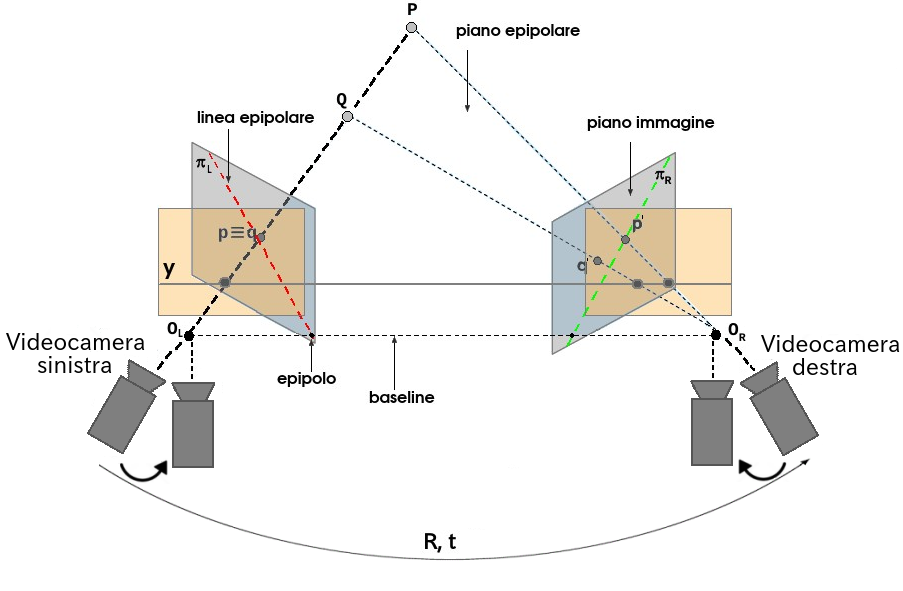
\includegraphics[width=1.1\linewidth]{./img/rect.png}
\begin{itemize}
\item[1.] \small{Calibrazione parametri intriseci ed estrinseci
\item[2.] Rettificazione
\item[3.] Calcolo delle corrispondenze
\item[4.] Computazione mappa di disparit\`{a}}
\end{itemize}
\end{column}
\begin{column}{5cm}
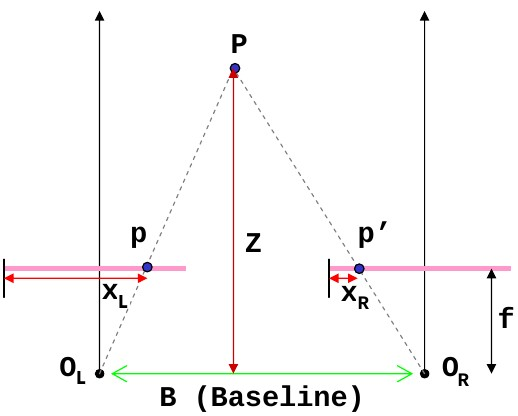
\includegraphics[width=0.8\linewidth]{./img/depth.jpg}
\begin{itemize}
\item \small{Triangolazione}:
\begin{center}
 $\frac{B}{Z} = \frac{(B+x_{L}) - x_{R}}{Z-f}$,
$Z = \frac{B \cdot f}{x_{L} - x_{R}} = \frac{B \cdot f}{d}$
\end{center}
\item  $\mathbf{d = x_{L} - x_{R}} $ \`{e} la \textbf{disparit\`{a}} 
\end{itemize}
\end{column}
\end{columns}
\end{frame}


% % % % % % % % % % FRAME % % % % % % % % % % % % %


\begin{frame}[t]{\textsc{Mappa di Disparit\`{a}: codifica}}
\begin{columns}
\hspace*{-4em}
\begin{column}{5cm}
\vspace{1em}
\begin{itemize}
\item  Codificata come un'immagine in scala di grigi
\item  Punti pi\`{u} vicini alla telecamera sono pi\`{u} chiari e corrispondono a una disparit\`{a} maggiore 
\end{itemize}
\end{column}
\hspace*{-3em}
\begin{column}{5.5cm}
\vspace{2em}
\centering
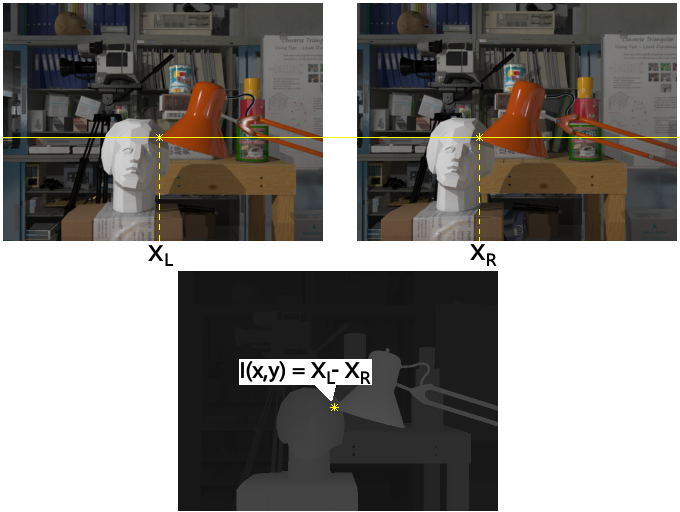
\includegraphics[width=1.2\linewidth]{./img/disparity.png}
\end{column}
\end{columns}
\end{frame}


% % % % % % % % % % FRAME % % % % % % % % % % % % %


\begin{frame}[t]{\textsc{Mappa di Disparit\`{a}: computazione}}
\begin{columns}
\begin{column}{5cm}
\vspace{1em}
\begin{itemize}
\item \small{\textbf{Metodi locali}: calcolare un valore di similarit\`{a} (MSE, NCC..) all'interno di una finestra  
\item \textbf{Metodi globali}: minimizzare su tutta l'immagine una funzione di energia che racchiude le assunzioni di corrispondenza
}
\end{itemize}
\end{column}
\begin{column}{5.5cm}
\vspace{1.5em}
\centering
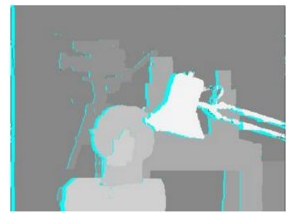
\includegraphics[width=1\linewidth]{./img/graph.png}
\end{column}
\end{columns}
\vspace{-1em}
\begin{center}
	\setbeamertemplate{blocks}[rounded][shadow=false]
	\setbeamercolor{block title}{use=structure,fg=black,bg=lightgray} 
	\setbeamercolor{block body}{use=structure,fg=black,bg=lightgray}
\begin{block}{}
\center \small{In questa tesi \`{e} stato utilizzato il metodo globale  di Kolmogorov and Zabih \textbf{Graph Cuts Stereo Matching Algorithm}}
\end{block}
\end{center}
\end{frame}


% % % % % % % % % % FRAME % % % % % % % % % % % % %


\subsection {Principi del watermarking}
\begin{frame}[t]{\textsc{Watermarking}}
\begin{columns}
\begin{column}{5cm}
\vspace{1em}
%	\setbeamertemplate{blocks}[rounded][shadow=false]
%	\setbeamercolor{block title}{use=structure,fg=black,bg=lightgray} 
%	\setbeamercolor{block body}{use=structure,fg=black,bg=lightgray}
%\begin{block}{}
%\center \small{Il \textbf{watermarking digitale} consiste nell'\textbf{inserimento} di \textbf{informazione} in contenuti  multimediali digitali in modo tale che questa informazione possa essere successivamente \textbf{estratta} o individuata per investigare possibili \textbf{manipolazioni} del contenuto ed eventuali violazioni del \textbf{copyright}}
%\end{block}
\textbf{Processo di marchiatura}
\begin{itemize}
\item Codifica di informazione nascosta in un contenuto originale
\item Distribuzione del contenuto
\item Ritrovamento del marchio
\end{itemize}
\textbf{Propriet\`{a}}
\begin{itemize}
\item Trasparenza
\item Robustezza (\small{compressione, view synthesis, distribuzione web})
\end{itemize}
\end{column}
\begin{column}{5cm}
\centering
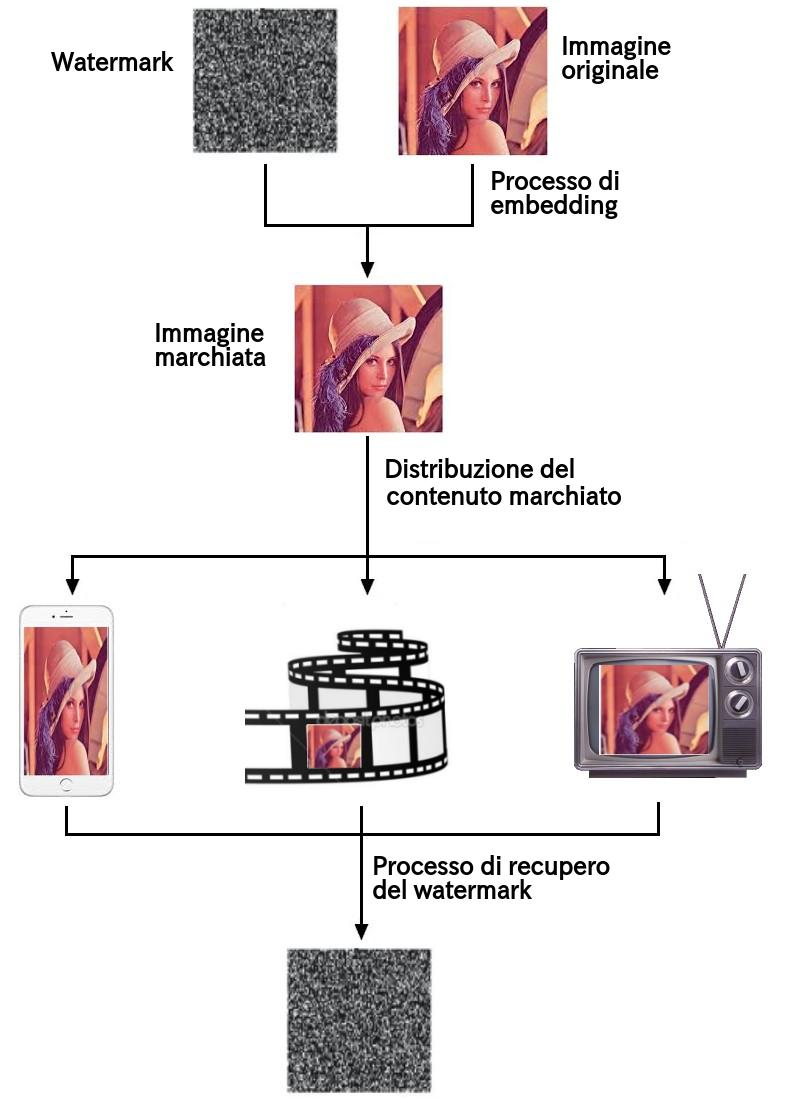
\includegraphics[width=1\linewidth]{./img/wat_workflow.jpg}
\end{column}
\end{columns}
\end{frame}

%\begin{frame}[t]{\textsc{Nozioni generali}}
%\begin{columns}
%\begin{column}{5cm}
%\vspace{1em}
%	\setbeamertemplate{blocks}[rounded][shadow=false]
%	\setbeamercolor{block body}{use=structure,fg=black,bg=lightgray}
%\begin{block}{Classificazione delle tecniche}
%\begin{itemize}
%\item Blind/Non blind
%\item Privata/Pubblica
%\item A lettura/A rilevamento
%\end{itemize}
%\end{block}
%\end{column}
%\begin{column}{5cm}
%\vspace{1em}
%	\setbeamertemplate{blocks}[rounded][shadow=false]
%	\setbeamercolor{block body}{use=structure,fg=black,bg=lightgray}
%\begin{block}{Requisiti del watermark}
%\begin{itemize}
%\item Trasparenza
%\item Robustezza
%\item Capacit\`{a}
%\end{itemize}
%\end{block}
%\end{column}
%\end{columns}
%\vspace{1em}
%\setbeamertemplate{blocks}[rounded][shadow=false]
%\setbeamercolor{block body}{use=structure,fg=black,bg=lightgray}
%\begin{block}{Domini e tecniche di inserimento}
%\begin{itemize}
%\item Spaziale/ Frequenza(DFT, DCT, DWT)
%\item Spread Spectrum/ Side Information
%\end{itemize}
%\end{block}
%\end{frame}

\subsection{Robustezza}
\vspace{2em}
\begin{frame}[t]{\textsc{View Synthesis}}
	\setbeamertemplate{blocks}[rounded][shadow=false]
	\setbeamercolor{block title}{use=structure,fg=black,bg=lightgray} 
	\setbeamercolor{block body}{use=structure,fg=black,bg=lightgray}
\begin{block}{}
\center \small{ Dato un insieme di immagini della stessa scena ottenute da diversi punti di vista, una \textbf{nuova immagine} viene \textbf{creata} considerando una \textbf{camera virtuale} posizionata in un diverso punto dello spazio}
\end{block}
\vspace{2em}
\centering
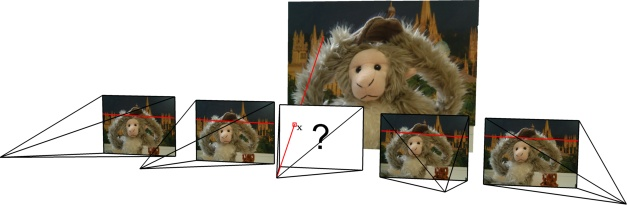
\includegraphics[width=1\linewidth]{./img/nvs.jpg}
\end{frame}

%\subsection{Tecniche di inserimento}
%\vspace{1em}
%\begin{frame}[t]{\textsc{Spread Spectrum nel dominio spaziale}}
%\begin{columns}
%\begin{column}{5cm}
%	\setbeamertemplate{blocks}[rounded][shadow=false]
%	\setbeamercolor{block body}{use=structure,fg=black,bg=lightgray}
%\vspace{1em}
%\begin{block}{Codifica}
%\centering Un pattern di rumore pseudo-random viene sommato al valore di luminanza di tutti i pixel dell'immagine
%$ \mathbf{I_{w}(x,y) = I(x,y) + \alpha w(x,y)}$
%\end{block}
%\begin{block}{Detection}
%Data l'immagine $\mathbf{I'}$ ritenuta marchiata viene calcolata la correlazione con il marchio $\mathbf{w}$
%\end{block}
%\end{column}
%\begin{column}{5cm}
%\vspace{1.5em}
%\centering
%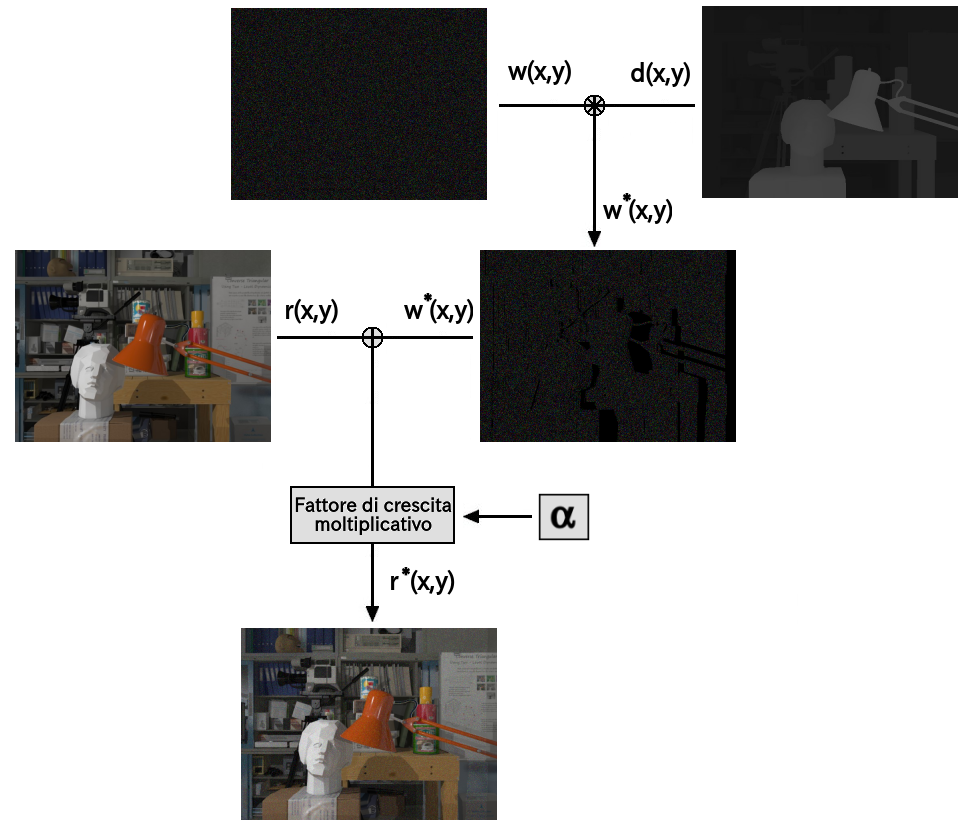
\includegraphics[width=1\linewidth]{./img/ss.png}
%\end{column}
%\end{columns}
%\end{frame}
%
%
%\subsection{Domini di inserimento}
%\begin{frame}[t]{\textsc{Inserimento in DFT}}
%\vspace{1em}
%\centering
%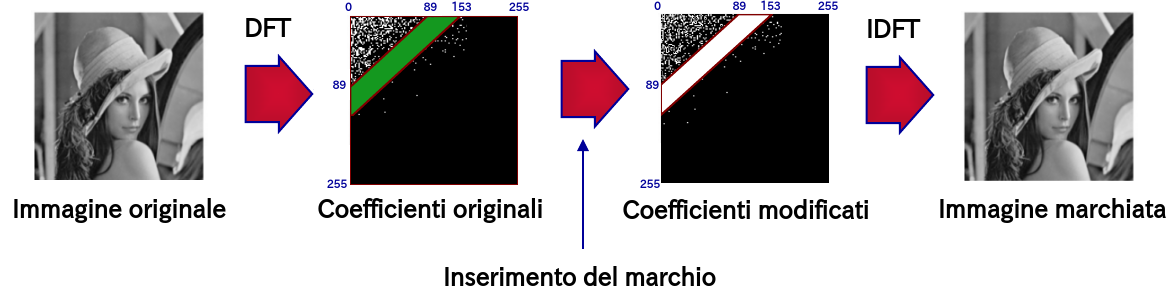
\includegraphics[width=1\linewidth]{./img/dft.png}
%\begin{itemize}
%\item Trasformazione immagine con Discrete Fourier Transform
%\item Selezione di n coefficienti $\mathbf{v_i}$ (medie frequenze)
%\item Generazione di una sequenza pseudo-random $\mathbf{w}$
%\item Modifica dei coefficienti: 
%\vspace{-2.3em}
% \begin{align*} 
%\qquad \mathbf{v'_{i} = v_i + \alpha w_{i}}\\
%		\mathbf{v'_{i} = v_i + \alpha v_i  w_{i}}
%\end{align*}
%\vspace{-2.5em}
%\item Ritorno al dominio spaziale con la trasformata inversa
%\end{itemize}
%\end{frame}

\subsection{Watermarking di video stereoscopici}

% % % % % % % % % % FRAME % % % % % % % % % % % % %


\begin{frame}[t]{\textsc{Metodi a Disparit\`{a} Coerente}}
\vspace{1em}
\centering

\begin{center}
\begin{itemize}

\item Marchiatura della \textbf{coppia stereo}
\item \textbf{Punti corrispondenti} nelle due viste presentano lo \textbf{stesso} campione del \textbf{marchio}
\item Il watermark viene modificato in base alla disparit\`{a} prima di essere inserito nella vista destra 
\item Vantaggi:
	\begin{itemize}
	\item Migliore \textbf{qualit\`{a} visiva}
	\item Maggior grado di \textbf{robustezza} contro attacchi di \textbf{view synthesis}
	\end{itemize}
\end{itemize}
\end{center}
\end{frame}
 
 
 % % % % % % % % % % FRAME % % % % % % % % % % % % %

\end{section}

\begin{section}{Marchiatura spaziale}
\subsection{Processo di codifica}
\begin{frame}[t]{\textsc{Marchiatura spaziale a disparit\`{a} coerente}}
\vspace{-2em}
\begin{columns}
\begin{column}{6cm}
	\setbeamertemplate{blocks}[rounded][shadow=false]
	\setbeamercolor{block body}{use=structure,fg=black,bg=lightgray}
\vspace{1em}
\begin{block}{Codifica vista sinistra}
\begin{itemize}
\item Metodo Spread Spectrum(\textbf{SS}):
\begin{center}
$\boldsymbol{l^{w} = l+\alpha w_{K}}$
\end{center}
\item Il marchio $\mathbf{w_{K}}$ segue $N(0, 1)$, $\boldsymbol{\alpha} \in \{1,3\}$
\end{itemize}
\end{block}
\begin{block}{Codifica vista destra}
\begin{itemize}
\item $\mathbf{w_{K}}$ deformato in base ai valori della disparit\`{a}:
\begin{center}
 $\boldsymbol{w^{*}_{K}(x,y) = w_{K}(x+d(x,y), y)}$
\end{center}
\item Inserito con SS:
$ \boldsymbol{r^{w} = r+\alpha w^{*}_{K}}$
\end{itemize}
\end{block}
\end{column}
\begin{column}{5cm}
\vspace{2em}
\begin{center}
\begin{figure}
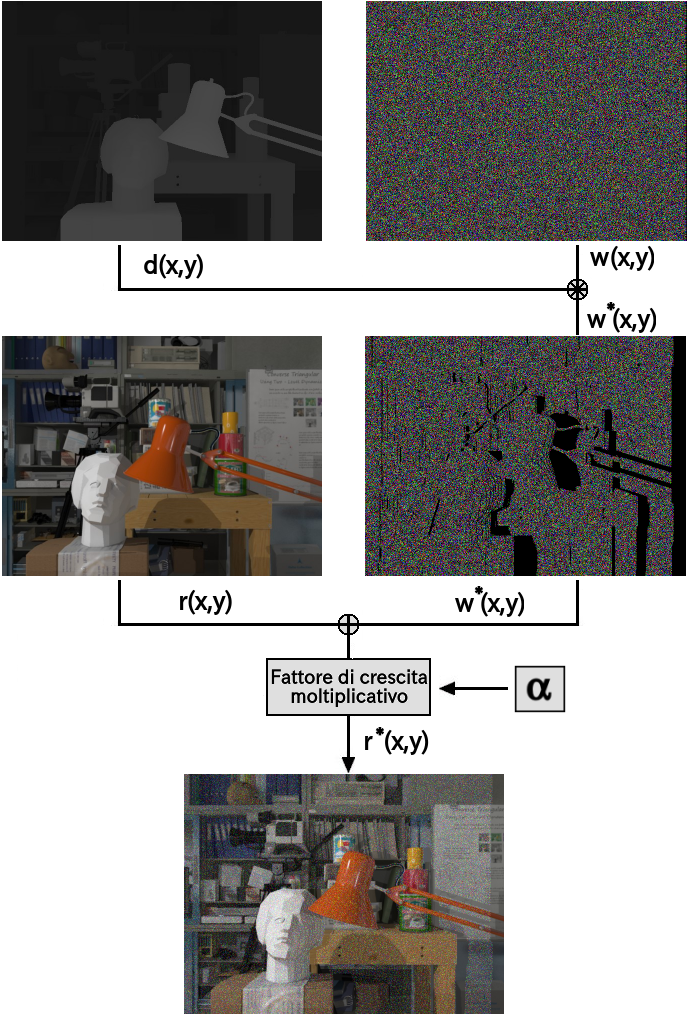
\includegraphics[width=0.9\linewidth]{./img/warp.png}
\end{figure}
\end{center}
\end{column}
\end{columns}
\end{frame}

% % % % % % % % % % FRAME % % % % % % % % % % % % %
\subsection{Processo di decodifica}
\begin{frame}[t]{\textsc{Marchiatura spaziale a disparit\`{a} coerente}}
\vspace{-0.5em}
\begin{columns}
\begin{column}{6cm}
	\setbeamertemplate{blocks}[rounded][shadow=false]
	\setbeamercolor{block body}{use=structure,fg=black,bg=lightgray}
\vspace{1em}
\begin{block}{Decodifica vista sinistra}
\begin{itemize}
\item Correlazione \textbf{vista sinistra} e \textbf{marchio originale}
\end{itemize}
\end{block}
\begin{block}{Decodifica vista destra}
\begin{itemize}
\item[1.] Correlazione \textbf{vista destra} e \textbf{marchio distorto}
\end{itemize}
\vspace{-0.5em}
oppure
\begin{itemize}
\item[2.] Correlazione \textbf{vista sinistra ricostruita} (attraverso vista destra e disparit\`{a}) e marchio originale
\end{itemize}
\end{block}
\end{column}
\begin{column}{5cm}
\vspace{2em}
\begin{center}
\begin{figure}
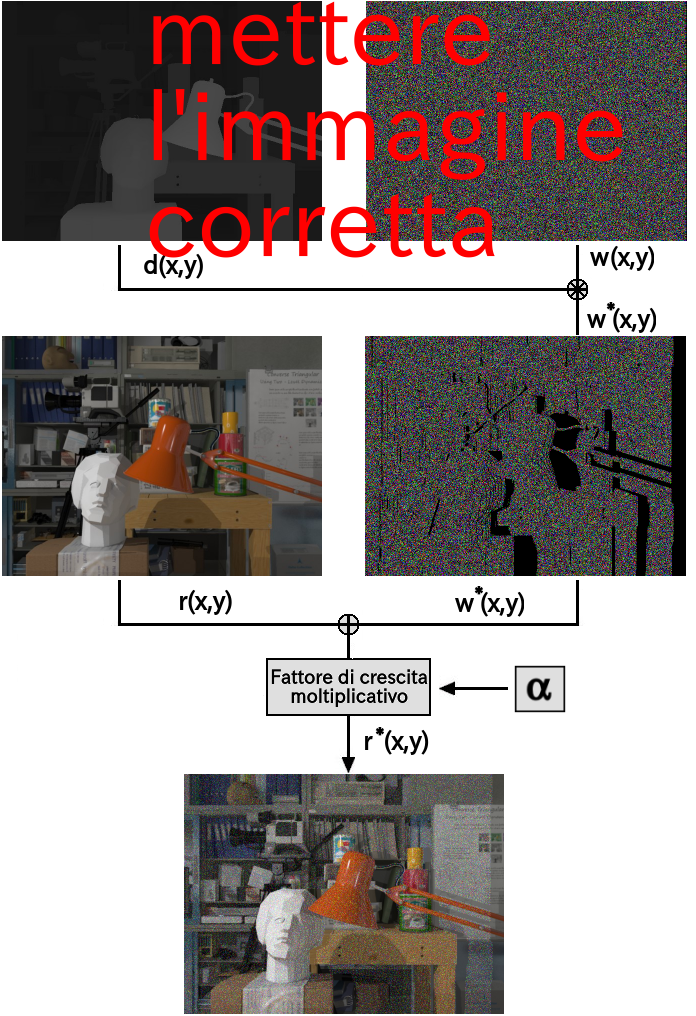
\includegraphics[width=0.9\linewidth]{./img/warp2.png}
\end{figure}
\end{center}
\end{column}
\end{columns}
\end{frame}

\end{section}

\begin{section}{Metodo in frequenza}

\begin{frame}[t]{\textsc{Algoritmo di marchiatura nel dominio della frequenza}}
\vspace{1em}
\centering
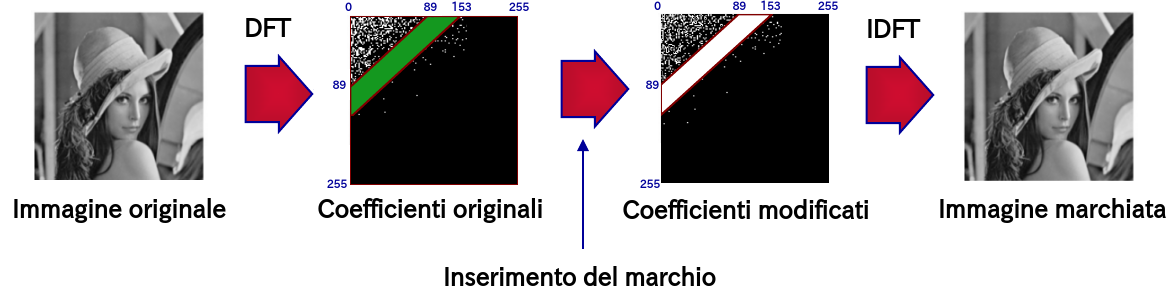
\includegraphics[width=1\linewidth]{./img/dft.png}
\begin{center}
\setbeamertemplate{blocks}[rounded][shadow=false]
%\setbeamercolor{block title}{use=structure,fg=black,bg=lightgray} 
\setbeamercolor{block body}{use=structure,fg=black,bg=lightgray} 
\begin{block}{Vantaggi:}
\center{\begin{itemize}
\item Visibilit\`{a}
\item Invariante a traslazioni
\item Resistente a degradazioni
\end{itemize}}
\end{block}
\end{center}
\end{frame}


\subsection{Processo di marchiatura stereo}

\begin{frame}[t]{\textsc{Marchiatura vista sinistra}}
\begin{figure}
  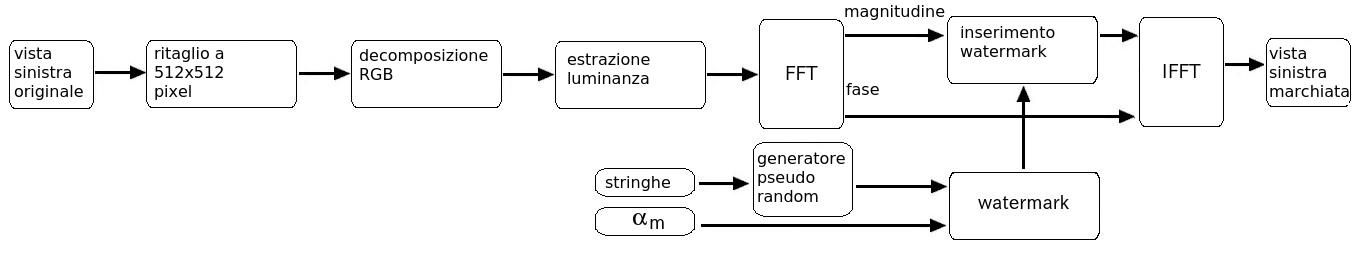
\includegraphics[width=1\textwidth]{./img_wat/left_wat.jpg}  
  \label{fig:leftwat}
\end{figure}

\begin{center}
\setbeamertemplate{blocks}[rounded][shadow=false]
%\setbeamercolor{block title}{use=structure,fg=black,bg=lightgray} 
\setbeamercolor{block body}{use=structure,fg=black,bg=lightgray} 
\begin{block}{Inserimento marchio:}
\center{\begin{itemize}
\item estrazione luminanza di $\mathbf{l}$
\item estrazione coefficienti a media frequenza
\item alterazione coefficienti: $\boldsymbol{v'_{l_{i}} = v_{l_{i}} + \alpha w_{i} v_{l_{i}} }$
\end{itemize}}
\end{block}
\end{center}

\end{frame}



\begin{frame}[t]{\textsc{Marchiatura vista destra}}
\begin{figure}
  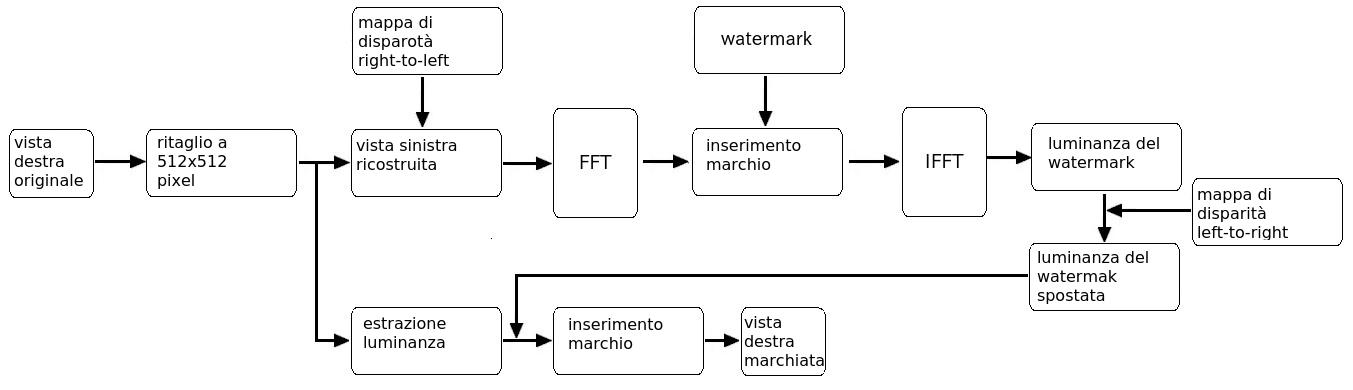
\includegraphics[width=0.95\textwidth]{./img_wat/pros.jpg}  
  \label{fig:rightwat}
\end{figure}
\setbeamertemplate{blocks}[rounded][shadow=false]
%\setbeamercolor{block title}{use=structure,fg=black,bg=lightgray} 
\setbeamercolor{block body}{use=structure,fg=black,bg=lightgray} 
\begin{block}{Obiettivi:}
\center{\begin{itemize}
\item Pixel corrispondenti marchiati nello stesso modo;
\item Marchio inserito spazialmente ma rilevabile in frequenza.
\end{itemize}}
\end{block}
\end{frame}

\begin{frame}[t]{\textsc{Marchiatura vista destra}}
\textbf{Idea}: 
\vspace{-0.8em}
\begin{figure}
  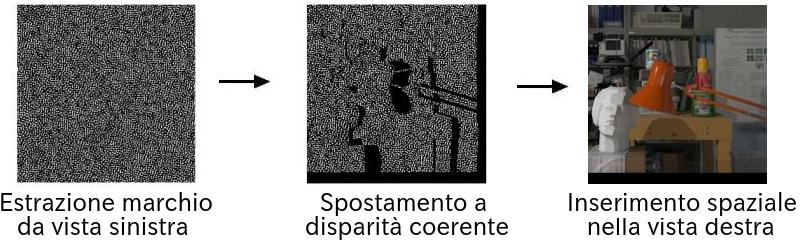
\includegraphics[width=0.75\textwidth]{./img_wat/idea.jpg}
  \label{fig:idea}
\end{figure}
\vspace{-3mm}
Se consideriamo l'immagine  $\mathbf{l}$ scritta in funzione della sua trasformata  $\mathbf{L}$ :
\begin{center}
  \scalebox{0.8}{%
$\boldsymbol{ l =  \frac{1}{MN}\sum\sum(|L(u,v)|)\exp\{\phi (u,v)\} e^{\{-j2\pi(\frac{ux}{M}+\frac{vy}{N})\}}  }$
  }
\end{center}
Dopo il processo di marchiatura: 
%\vspace{-1.5em}
\begin{center}
  \scalebox{0.8}{%
$\boldsymbol{ l_{w} = \frac{1}{MN}\sum\sum(|L(u,v)| + \alpha|L(u,v)||w|)e^{\{j(\phi_{L}+\phi{w})\}}e^{\{-j2\pi(\frac{ux}{M}+\frac{vy}{N})\}}} $
  }
\end{center}

\end{frame}

\begin{frame}[t]{\textsc{Marchiatura vista destra}}
\setbeamertemplate{blocks}[rounded][shadow=false]
%\setbeamercolor{block title}{use=structure,fg=black,bg=lightgray} 
\setbeamercolor{block body}{use=structure,fg=black,bg=lightgray} 
\begin{block}{Problemi:}
\center{\begin{itemize}
\item La procedura di detection si aspetta in ingresso un'immagine del tipo:
%\vspace{1em}
\begin{center}
  \scalebox{0.8}{%
$\boldsymbol{ r_{w} = r + \frac{1}{MN}\sum\sum(\alpha|R(u,v)||w|e^{\{j(\phi_{R}+\phi{w})\}})e^{\{-j2\pi(\frac{ux}{M}+\frac{vy}{N})\}}} $
  }
\end{center}
\item L'alterazione estratta dalla vista sinistra \`{e} del tipo:
%\vspace{-2mm}
\begin{center}
  \scalebox{0.8}{%
$\boldsymbol{ \alpha|L||w|e^{\{j(\phi_{L}+\phi{w})\}}} $
  }
\end{center}
\end{itemize}}
\end{block}
\begin{block}{Soluzione:}
		\begin{itemize}
		\item \textbf{modulo} \textbf{marchio}: modulo della vista sinistra ricostruita a partire dai pixel della vista destra;
		\item \textbf{fase} \textbf{marchio}: fase della vista sinistra sommata a quella del marchio di riferimento; 
		\end{itemize}
\end{block}

\end{frame}


\begin{frame}[t]{\textsc{Marchiatura vista destra}}
\vspace{5mm}
Il marchio inserito nella vista destra \`{e} quindi:
\begin{center}
  \scalebox{1}{%
$\boldsymbol{  \alpha|R^{**}||w|e^{\{j(\phi_{L}+\phi{w})\}} }$
  }
\end{center}
\vspace{3mm}
Le formule complete sono:
\vspace{3mm}
\setbeamertemplate{blocks}[rounded][shadow=false]
%\setbeamercolor{block title}{use=structure,fg=black,bg=lightgray} 
\setbeamercolor{block body}{use=structure,fg=black,bg=lightgray} 
\begin{block}{}
\begin{center}
  \scalebox{0.9}{%
$\boldsymbol{ l_{w} = l + \frac{1}{MN}\sum\sum(\alpha|L(u,v)||w|e^{\{j(\phi_{L}+\phi_{w})\}})e^{\{-j2\pi(\frac{ux}{M}+\frac{vy}{N})\}} }$

  }
\end{center}
\begin{center}
  \scalebox{0.9}{%

$\boldsymbol{ r_{w} = r + \frac{1}{MN}\sum\sum(\alpha|R(u,v)^{**}||w|e^{\{j(\phi_{L}+\phi_{w})\}})^{*}e^{\{-j2\pi(\frac{ux}{M}+\frac{vy}{N})\} }}$
  }
\end{center}
\end{block}
\end{frame}


\begin{frame}[t]{\textsc{Detection vista sinistra}}

\begin{figure}
  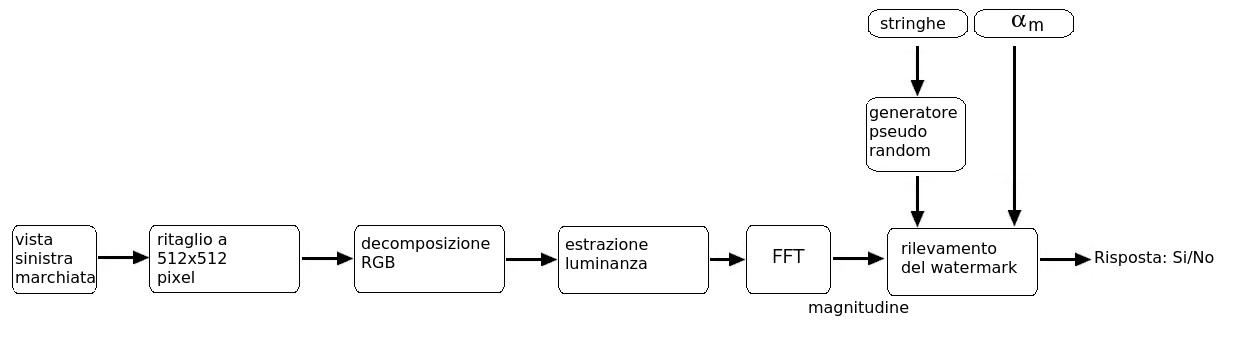
\includegraphics[width=0.95\textwidth]{./img_wat/left_det.jpg}
  
  \label{fig:leftdet}
\end{figure}
\setbeamertemplate{blocks}[rounded][shadow=false]
%\setbeamercolor{block title}{use=structure,fg=black,bg=lightgray} 
\setbeamercolor{block body}{use=structure,fg=black,bg=lightgray} 
\begin{block}{Detection basata su soglia:}
\center{\begin{itemize}
\item generazione marchio;
\item calcolo likelihood $\mathbf{L(y)}$ e soglia $\boldsymbol{\lambda}$ con il criterio di Neyman-Pearson;
\item comparazione $\mathbf{L(y)}$ con $\boldsymbol{\lambda}$ e decisione.
\end{itemize}}
\end{block}
\end{frame}

\begin{frame}[t]{\textsc{Detection vista destra}}
\begin{figure}
  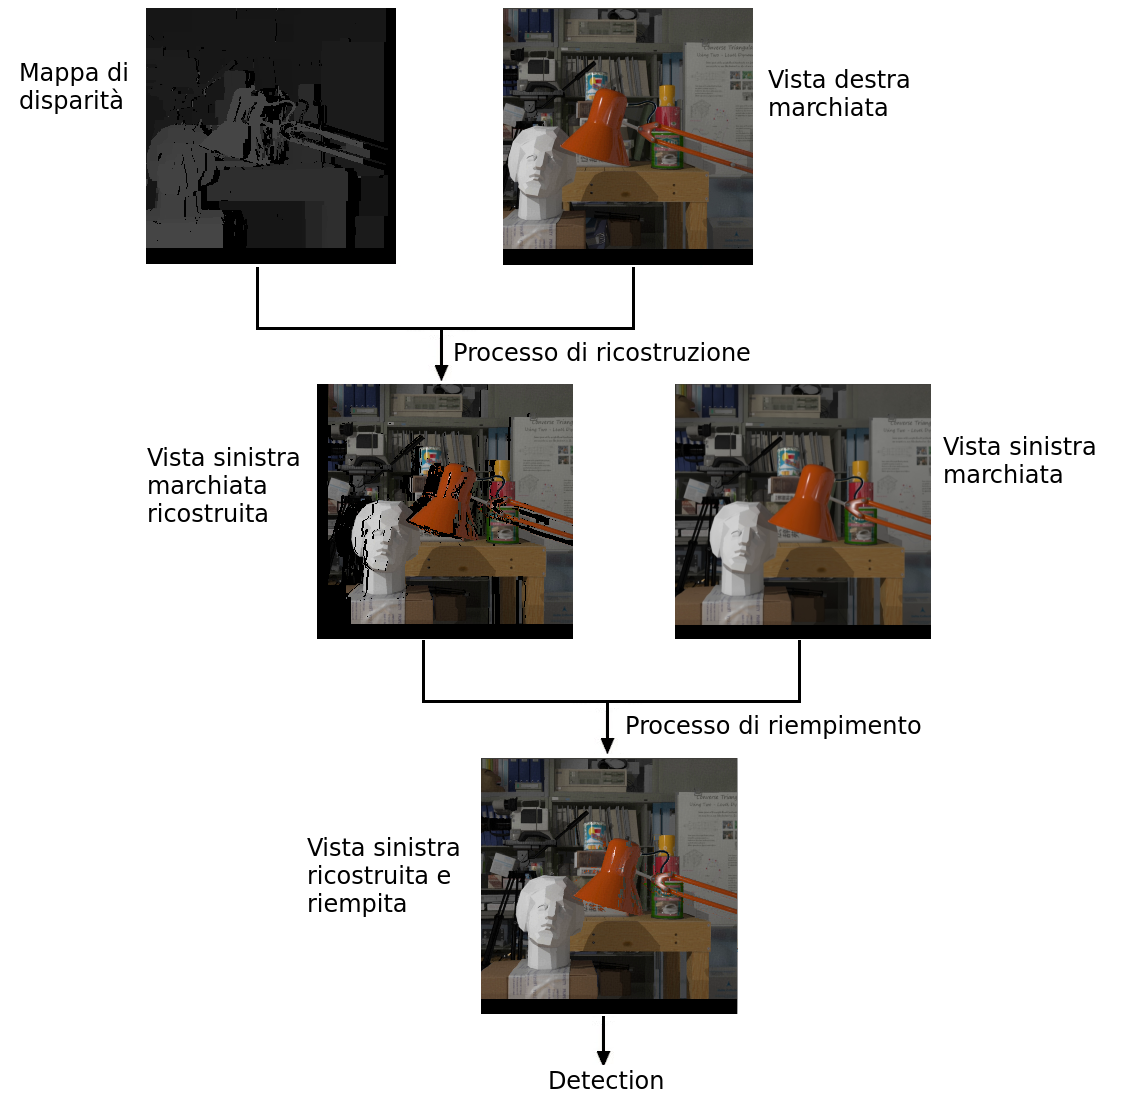
\includegraphics[width=0.65\textwidth]{./img_wat/detection_workflow.png}  
  \label{fig:rightdetflow}
\end{figure}
\end{frame}

\end{section}

\begin{section}{Risultati sperimentali}

\begin{frame}[t]{\textsc{Risultati sperimentali}}
Test effettuati su:
\begin{itemize}
\item sequenza video di 1 minuto creata dal \textbf{dataset Tsukuba}
\item frame stereo 1280x480
\item frame rate 30
\item group of picture 60
\end{itemize}

\vspace{2mm}
\begin{figure}
  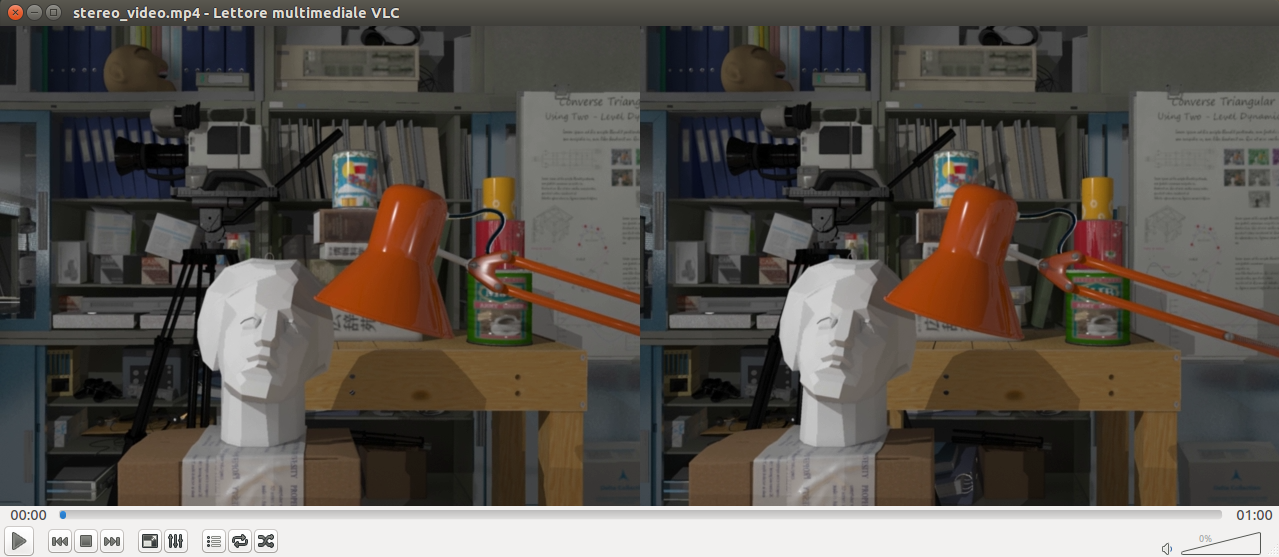
\includegraphics[width=0.8\textwidth]{./img_wat/video_stereo.png}  
  \label{fig:video}
\end{figure}
\end{frame}

\subsection{Risultati sperimentali}

\begin{frame}[t]{\textsc{Test di robustezza}}
\setbeamertemplate{blocks}[rounded][shadow=false]
%\setbeamercolor{block title}{use=structure,fg=black,bg=lightgray} 
\setbeamercolor{block body}{use=structure,fg=black,bg=lightgray} 
\begin{block}{Compressione:}
Si studia la degradazione del marchio dovuta alla compressione del video, in relazione alla potenza di inserimento.
\end{block}
\begin{block}{Distribuzione web:}
Si studia la resistenza del marchio in video che sono stati caricati su Youtube e successivamente scaricati.
\end{block}
\begin{block}{Sintetizzazione di viste intermedie:}
Si studia la risposta del marchio in caso di creazione di viste sintetiche a tre diverse distanze dalla vista sinistra.
\end{block}

\end{frame}

\begin{frame}[t]{\textsc{Compressione}}
\vspace{-2mm}
\begin{table}
\scalebox{0.6}{
\begin{tabular}{c | c | c }
potenza marchio & livello di compressione & Detection stereo \\
\hline \hline
\rowcolor{LRed}  \textbf{1} & \textbf{1} & \textbf{70\%} \\
1 & 15 & 40\%\\
 1 & 25 & $< 20\% $\\
 1 & 30 & $< 20\% $ \\\hline
 3 & 1 &  $ >80\% $\\
\rowcolor{LRed} \textbf{3} & \textbf{15} &  $ \boldsymbol{70\%} $\\
 3 & 25 & $ 30\% $\\
 3 & 30 &  $ <20\% $ \\\hline

\end{tabular}
}

\end{table}
\begin{center}
\scalebox{0.7}{Statistica della detection spaziale}
\end{center}
\vspace{-2mm}
\begin{table}
\scalebox{0.6}{
\begin{tabular}{c | c | c }
potenza marchio & livello di compressione & Detection stereo \\
\hline \hline
 0.3 & 1 & 100\% \\
\rowcolor{LRed} \textbf{0.3} & \textbf{15} & $\boldsymbol{>96\%} $\\
 0.3 & 25 & 36.6\%  \\
 0.3 & 30 & 6.6\% \\\hline
 0.6 & 1 & 100\%  \\
 0.6 & 15 & 100\%  \\
\rowcolor{LRed} \textbf{0.6} & \textbf{25} & \textbf{86.6\%} \\
 0.6 & 30 & 50\% \\
\end{tabular}
}
\end{table}
\begin{center}
\scalebox{0.7}{Statistica della detection in frequenza}
\end{center}
\end{frame}



\begin{frame}[t]{\textsc{Distribuzione web}}
\begin{table}
\scalebox{0.75}{
\begin{tabular}{c | c }
livello di compressione & PSNR(dB) \\
\hline \hline
15 		    & 46.0194 \\
25 		    & 40.4861 \\
\rowcolor{LRed} \textbf{YT} 		    & \textbf{38.2039} \\
30 		    & 37.5587 \\
\end{tabular}
}
\vspace{2mm}
\caption{Valore medio di PSNR per diversi livelli di compressione}
\end{table}
\begin{table}
\scalebox{0.75}{
\begin{tabular}{c | c }
potenza del marchio & Detection stereo \\
\hline \hline
0.3 & $<20\%$ \\
0.5 & 20\% \\
\rowcolor{LRed} \textbf{0.6} & \textbf{37\%}\\
\end{tabular}
}
\vspace{2mm}
\caption{Statistica della detection in frequenza per video caricati su Youtube}
\end{table}

\end{frame}
\begin{frame}[t]{\textsc{Sintetizzazione di viste intermedie}}

\begin{figure}
  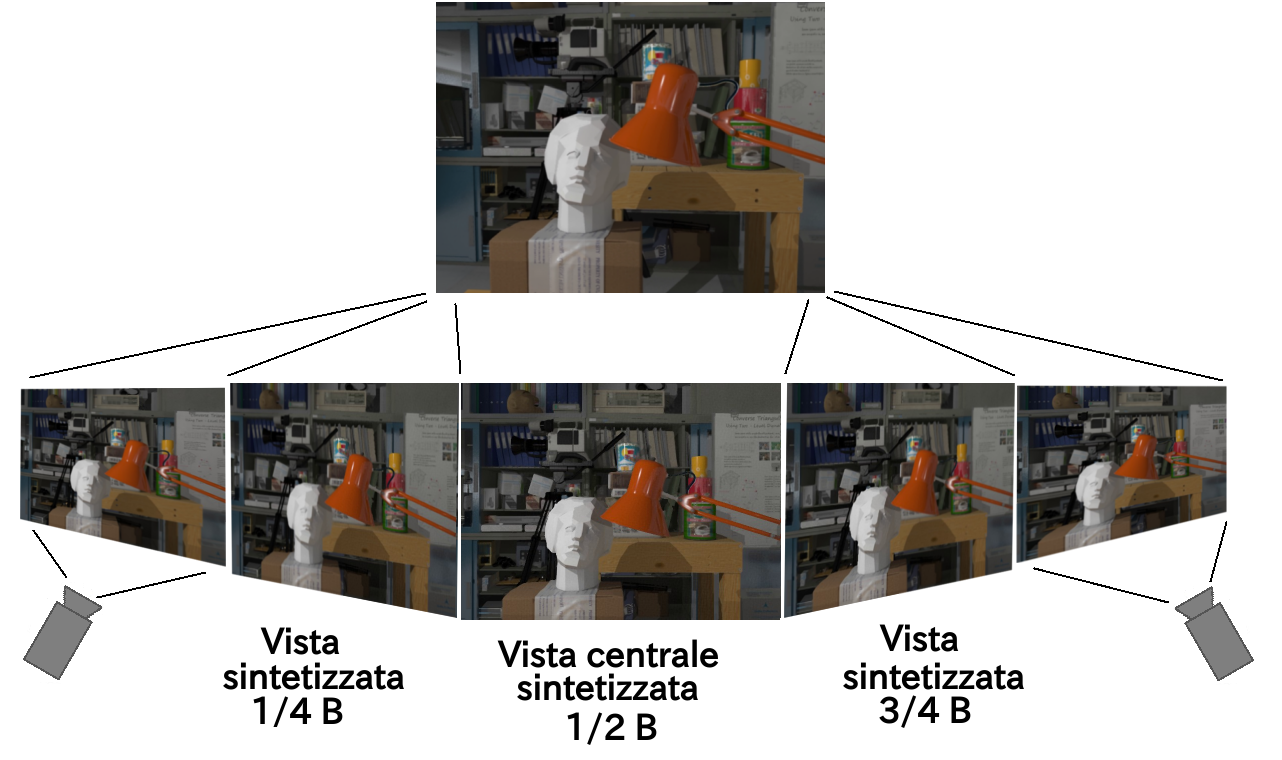
\includegraphics[width=0.6\textwidth]{./img/sintesi.png}  
  \caption{} 
  \label{fig:vsg1}
\end{figure}
\vspace{-3em}
\begin{table}
\scalebox{0.9}{
\begin{tabular}{c  c  c 	c }
 & vista 1/4B & vista 1/2B & vista 3/4B \\
\hline
Detection spaziale & $>90\%$  & $>80\% $  & $>80\% $  \\
Detection in frequenza & 100\% & 100\% & $>90\%$ \\	
\end{tabular}
}
\end{table}


\end{frame}



\begin{frame}[t]{\textsc{Test di trasparenza: misure di qualit\`{a} }}
\vspace{-13mm}
\begin{columns}
\begin{column}{5cm}
\begin{center}
\vspace{10mm}
\begin{figure}
  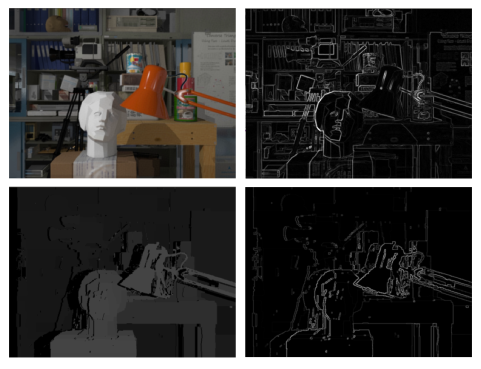
\includegraphics[width=1\textwidth]{./img_wat/quality.png}  
  \caption{} 
  \label{fig:qm}
\end{figure}
\end{center}
\end{column}
\begin{column}{5cm}
\vspace{-8mm}
\begin{center}
  \scalebox{0.65}{%
$ Q_{View}(x,y) = [l(x,y)]^{\alpha} \cdot [c(x,y)]^{\beta} \cdot [\mathbf{{S}_{View}(x',y')]^{\gamma}} $
  }
\end{center}

\vspace{1mm}
\begin{center}

  \scalebox{0.65}{%
$ Q_{Depth}(x,y) = [l(x,y)]^{\alpha} \cdot [c(x,y)]^{\beta} \cdot [\mathbf{{S}_{Depth}(x',y')]^{\gamma}} $
  }
\end{center}

\end{column}

\end{columns}
\vspace{-7mm}
\setbeamertemplate{blocks}[rounded][shadow=false]
%\setbeamercolor{block title}{use=structure,fg=black,bg=lightgray} 
\setbeamercolor{block body}{use=structure,fg=black,bg=lightgray} 

\begin{block}{\small Metriche di Chamida et al.}
\begin{itemize}
\item \small Basate sugli \textbf{edge} della mappa di disparit\`{a} e della vista da esaminare
\item \small Versione modificata di \textbf{SSIM} 
\item \small Metrica di tipo \textbf{Reduced-Reference} 
\end{itemize}
\end{block}
\end{frame}


\begin{frame}[t]{\textsc{Test di trasparenza: misure di qualit\`{a} }}
\vspace{-3mm}
\begin{figure}
  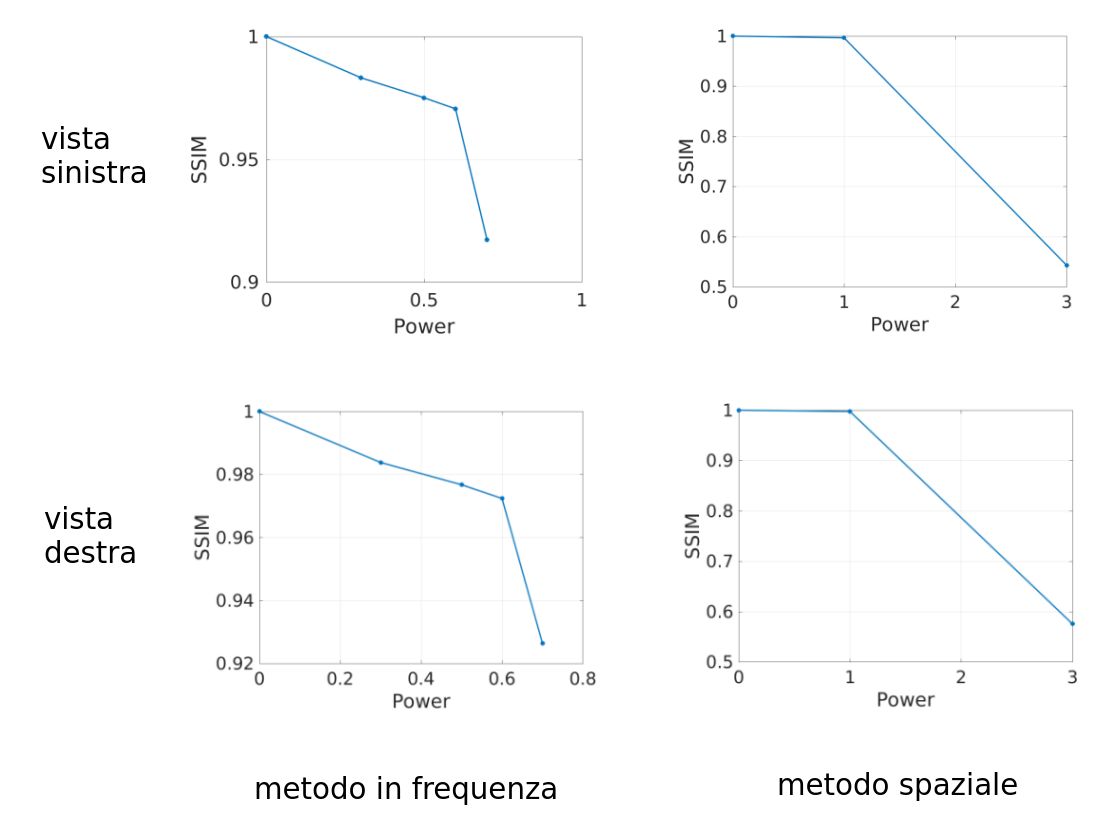
\includegraphics[width=0.9\textwidth]{./img_wat/qm_res.png}  
  \caption{} 
  \label{fig:qmgr}
\end{figure}


\end{frame}

\begin{frame}[t]{\textsc{Test di trasparenza: PSNR}}
\setbeamertemplate{blocks}[rounded][shadow=false]
\setbeamercolor{block title}{use=structure,fg=black,bg=lightgray} 
\setbeamercolor{block body}{use=structure,fg=black,bg=lightgray} 
\begin{block}{}

\begin{itemize}
\item Si \`{e} misurato l'impatto visivo tramite PSNR tra i frame originali e marchiati, al variare della potenza del marchio
\item valori tipici per video marchiati sono tra 30 e 50 dB
\end{itemize}
\end{block}
\vspace{4mm}
\begin{table}
\scalebox{0.8}{
\begin{tabular}{c | c }
potenza del marchio & PSNR(dB) \\
\hline \hline
0.3 		    & 46.0071 \\
0.5		    & 45.9505 \\
\textbf{0.6}		    & \textbf{45.9291} \\
\end{tabular}
}

\end{table}
\end{frame}

\end{section}

\begin{section}{Conclusioni}
\subsection{Conclusioni}


\begin{frame}[t]{\textsc{Conclusioni}}
Nel dominio spaziale:
\begin{columns}
\begin{column}{5cm}
\setbeamertemplate{blocks}[rounded][shadow=false]
\setbeamercolor{block title}{use=structure,fg=black,bg=lightgray} 
\setbeamercolor{block body}{use=structure,fg=black,bg=lightgray} 
\begin{block}{}
\begin{itemize}
\item fissiamo un degrado della qualit\`{a} dell'immagine del 1\%
\item otteniamo la potenza del marchio pari a 1
\end{itemize}
\end{block}
\end{column}

\begin{column}{5cm}
\vspace{-6mm}
\begin{table}
\scalebox{0.65}{
\begin{tabular}{c | c | c }
CRF & potenza del marchio & True positive \\
\hline \hline
\rowcolor{LRed}\textbf{ 1} & \textbf{1} & \textbf{70\%}\\
15 & 1 & 40\%\\
25 & 1 & $< 20\% $\\
30 & 1 & $< 20\% $\\
\end{tabular}
}
\end{table}

\end{column}
\end{columns}
\vspace{2mm}
\begin{figure}
  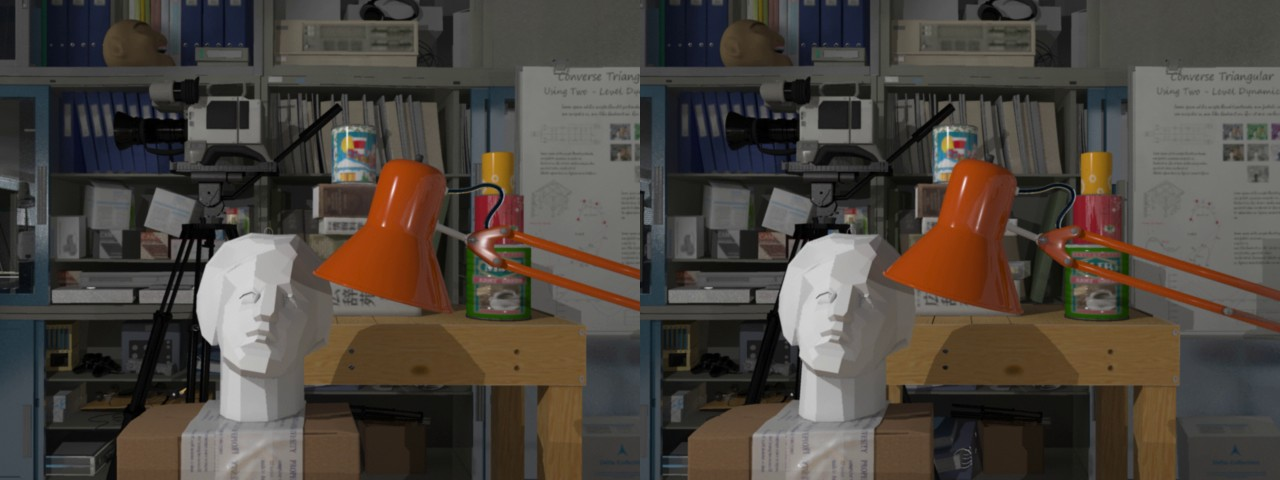
\includegraphics[width=0.7\textwidth]{./img_wat/marked_1_gauss.jpg}  
  \caption{} 
  \label{fig:mg1}
\end{figure}
\end{frame}


\begin{frame}[t]{\textsc{Conclusioni}}
Nel dominio della frequenza:
\begin{columns}
\begin{column}{5cm}
\setbeamertemplate{blocks}[rounded][shadow=false]
\setbeamercolor{block title}{use=structure,fg=black,bg=lightgray} 
\setbeamercolor{block body}{use=structure,fg=black,bg=lightgray} 
\begin{block}{}
\begin{itemize}
\item fissiamo un degrado della qualit\`{a} dell'immagine del 1\%
\item otteniamo la potenza del marchio pari a 0.3 
\end{itemize}
\end{block}

\end{column}
\begin{column}{5cm}
\vspace{-10mm}
\begin{table}
\scalebox{0.65}{
\begin{tabular}{c | c | c }
CRF & potenza del marchio & detection stereo \\
\hline \hline
1 & 0.3 & 100\%\\
\rowcolor{LRed} \textbf{15} & \textbf{0.3} & $\boldsymbol{>90\%}$\\
25 & 0.3 & 36.6\%\\
30 & 0.3 & 6.6\%\\
\end{tabular}
}
\end{table}

\end{column}
\end{columns}
\vspace{2mm}
\begin{figure}
  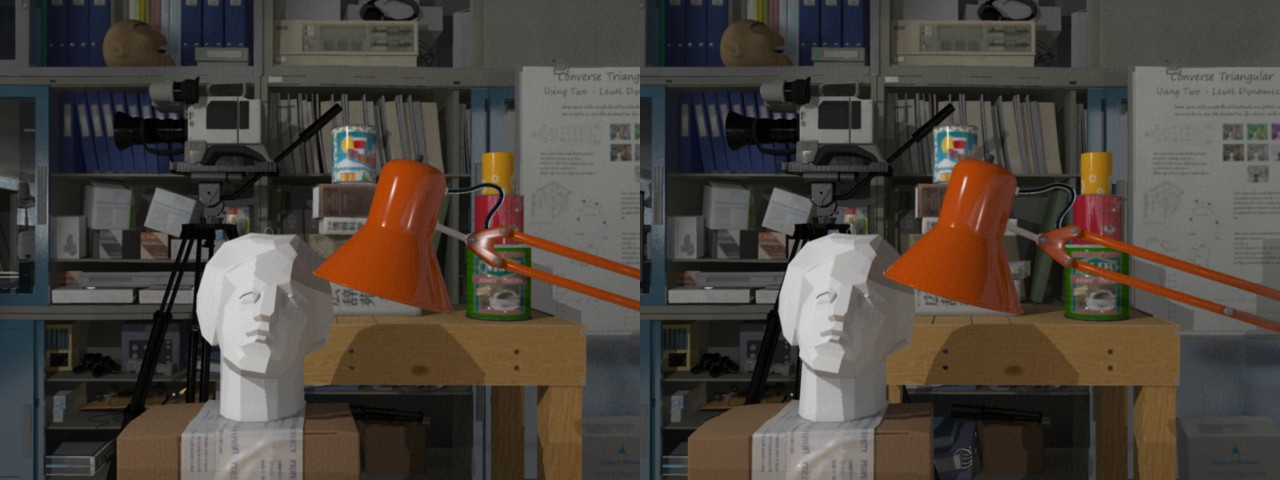
\includegraphics[width=0.7\textwidth]{./img_wat/marked_03_DFT.jpg}  
  \caption{} 
  \label{fig:mg1}
\end{figure}
\end{frame}



\begin{frame}[t]{\textsc{Video stereo marchiato con potenza 0.3 compresso a fattore 15
}}
\vspace{2mm}
\begin{center}
\movie[width=8cm,height=6cm,autostart,loop,poster]{}{./img_wat/anaglifico_03_kz.mkv}
\end{center}

\end{frame}
\end{section}



\end{document}
